\section{Web App}

\subsection{Requisiti}
Per poter utilizzare correttamente la web app è necessario disporre di una connessione ad internet e di un browser web che supporti l'estensione Metamask. L'applicazione è stata testata sui seguenti browser:
\begin{itemize}
    \item Google Chrome v112;
    \item Mozilla Firefox v112;
    \item Microsoft Edge v112.
\end{itemize}
L'unico tra i principali browser che non supporta Metamask è Safari, pertanto non è possibile utilizzare la web app su tale browser.

\subsubsection{MetaMask}
Per poter utilizzare la web app è necessaria un'installazione funzionante dell'estensione MetaMask per il browser web.

MetaMask è un portafoglio digitale che permette di interagire con la blockchain Ethereum e con gli smart contract eseguiti su di essa, offrendo la possibilità di effettuare transazioni con diverse criptovalute.

Per le istruzioni di installazione e configurazione di MetaMask si rimanda alla \href{https://support.metamask.io/hc/en-us/articles/360015489531-Getting-started-with-MetaMask}{documentazione ufficiale}.

\subsection{Funzionalità}
All'apertura della web app, verrà visualizzata la pagina principale. Come mostrato in \hyperref[fig:home]{Figura 1}, maggior parte delle funzionalità sarà disponibile solo dopo aver effettuato l'accesso con MetaMask; i bottoni corrispondenti a tali features saranno disabilitati fino ad allora.

% VERSIONE SODDISFACENTE
\begin{figure}[t]
    \centering
    \begin{subfigure}{0.4\textwidth}
    \centering
    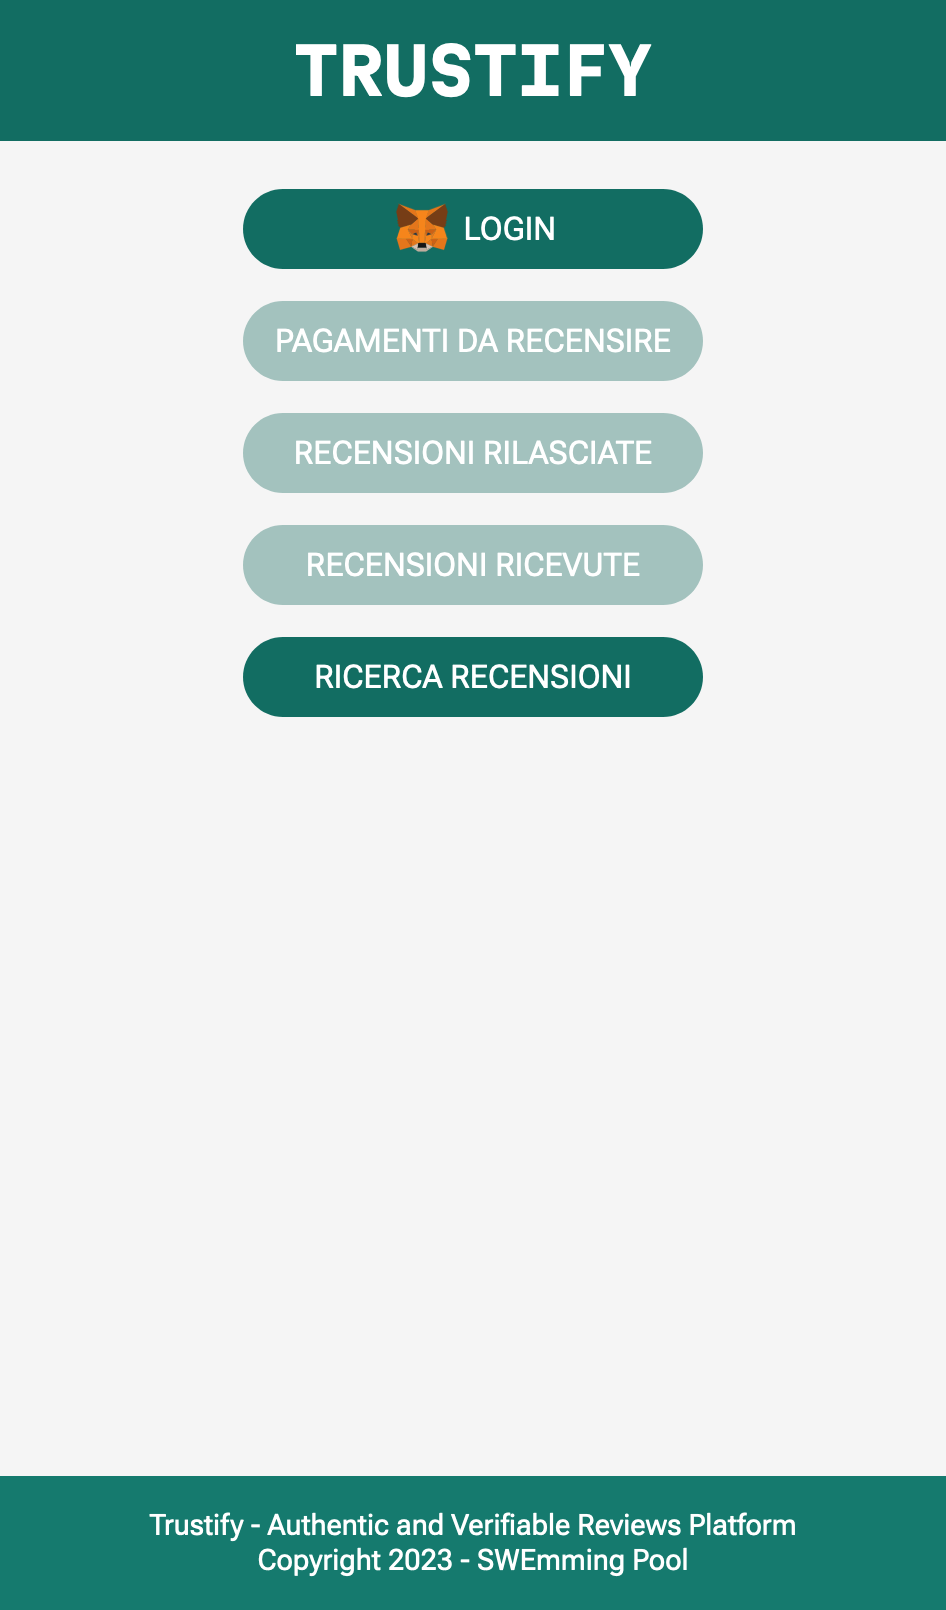
\includegraphics[width=0.9\linewidth]{src/img/home.png}
    \caption{Login non effettuato}\label{fig:home_nologin}
    \end{subfigure}
    \begin{subfigure}{0.4\textwidth}
    \centering
    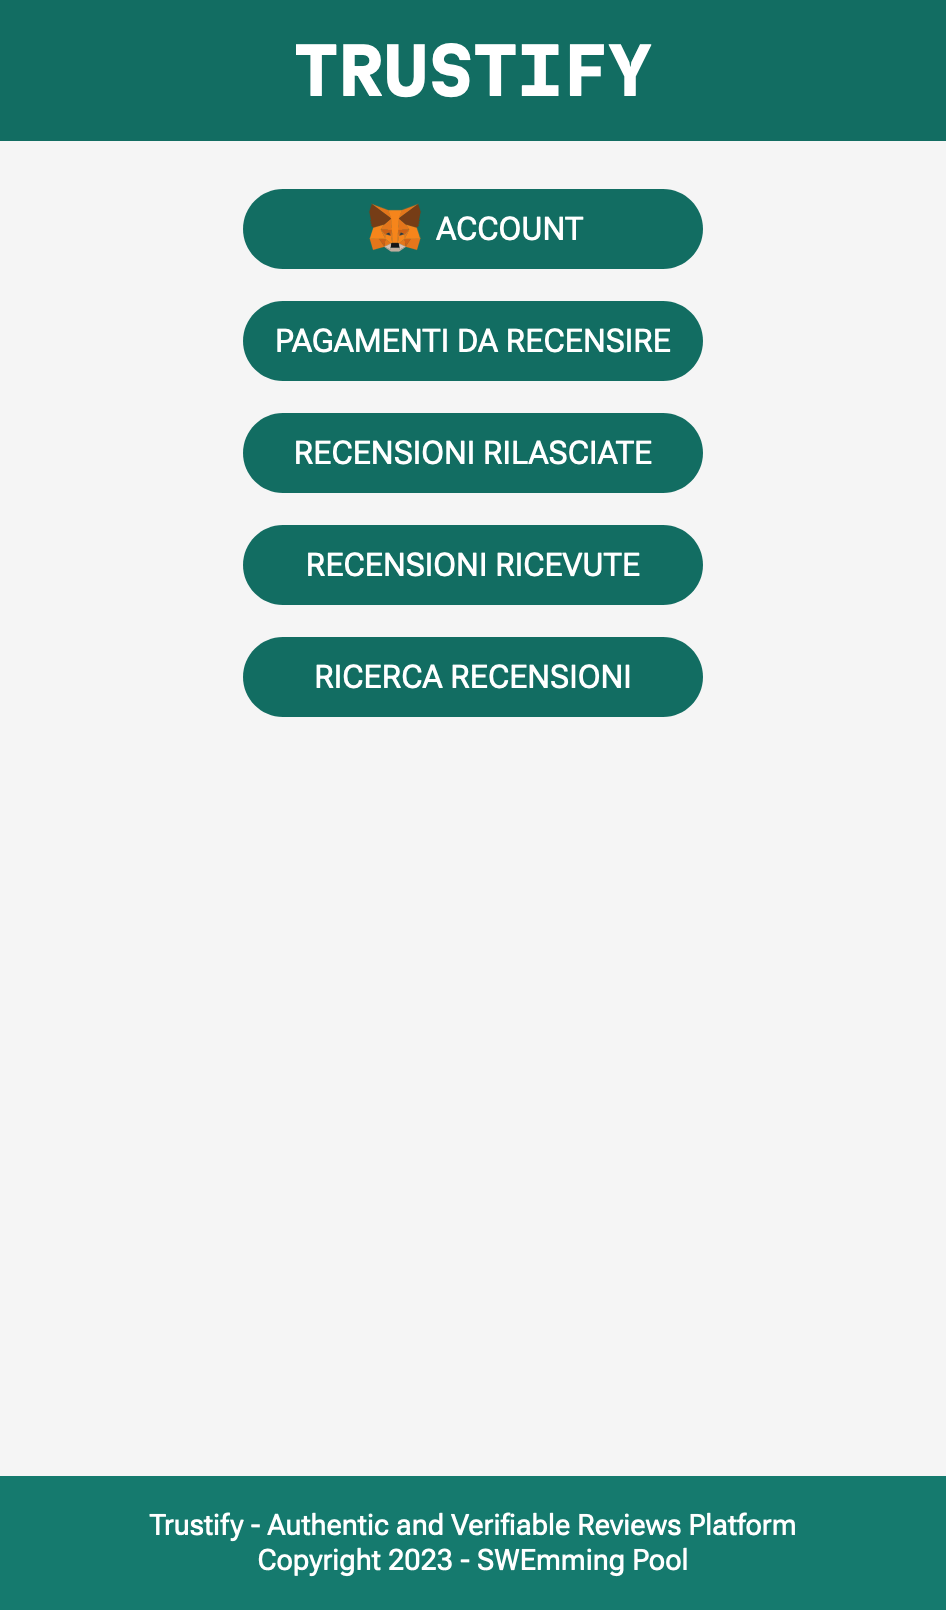
\includegraphics[width=0.9\linewidth]{src/img/home_login.png}
    \caption{Login effettuato}\label{fig:home_login}
    \end{subfigure}

    \caption{Pagina Home}\label{fig:home}
\end{figure}

Non è presente un bottone per effettuare pagamenti, in quanto il checkout, nella versione finale, sarà integrato direttamente nel sito web del commerciante, e dati quali indirizzo e prezzo da pagare non saranno modificabili dall'utente. È comunque possibile testare la funzionalità di pagamento come spiegato di seguito.

\subsubsection{Checkout}
Per motivi di test, è stato implementato un checkout di prova, accessibile inserendo nell'URL indirizzo del destinatario e quantità di ETH da inviare. Se, per esempio, la web app fosse hostata su \path{https://trustify.com}, l'URL avrebbe la seguente forma: \path{https://trustify.com/checkout/indirizzo-wallet/quantita-eth}.

Cliccando sul bottone "Paga con Trustify", verrà aperta una finestra di Metamask per confermare la transazione, e si sarà reindirizzati all'interno della web app. Una volta confermata, verrà visualizzata una pagina di conferma del pagamento.

\begin{figure}[t]
    \begin{subfigure}{0.33\textwidth}
    \centering
    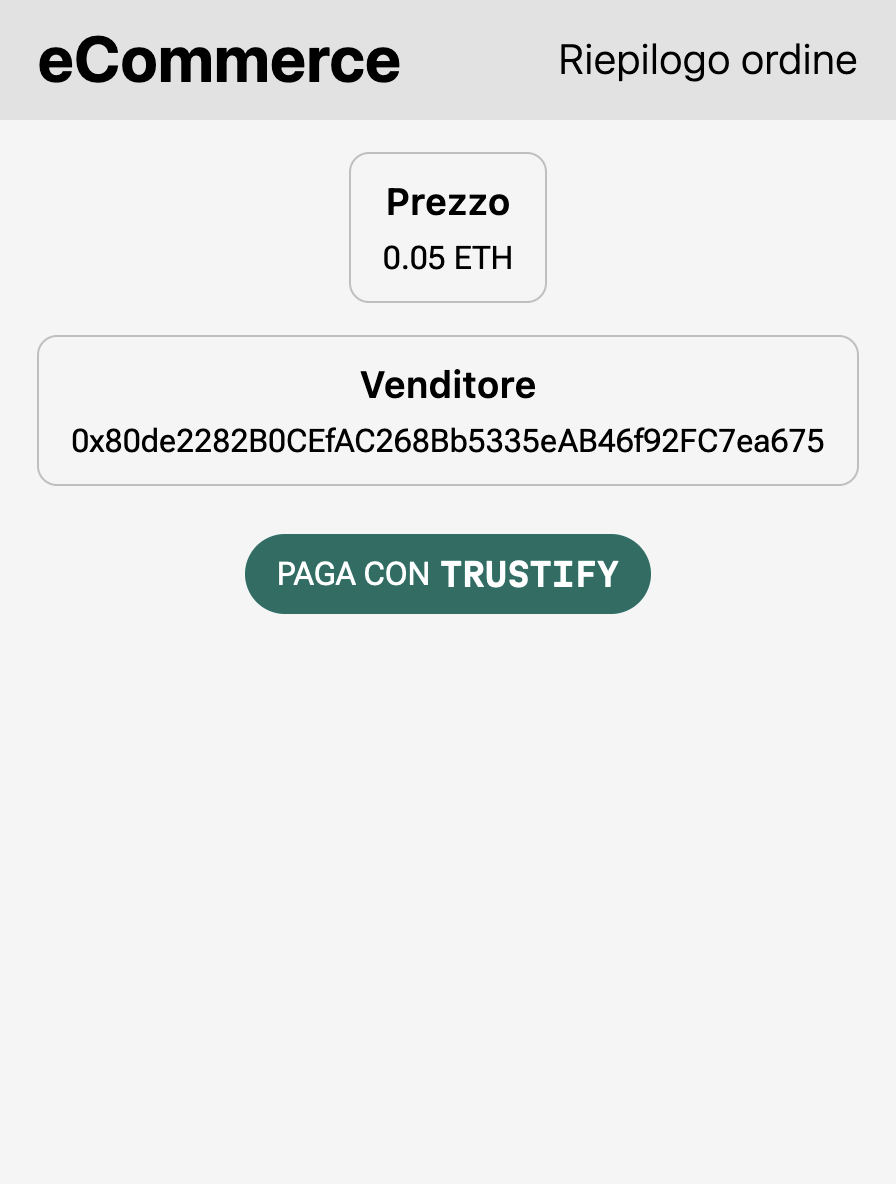
\includegraphics[width=0.9\linewidth]{src/img/checkout.png}
    \caption{Pagina di checkout fittizia}\label{fig:checkout_page}
    \end{subfigure}
    \begin{subfigure}{0.33\textwidth}
    \centering
    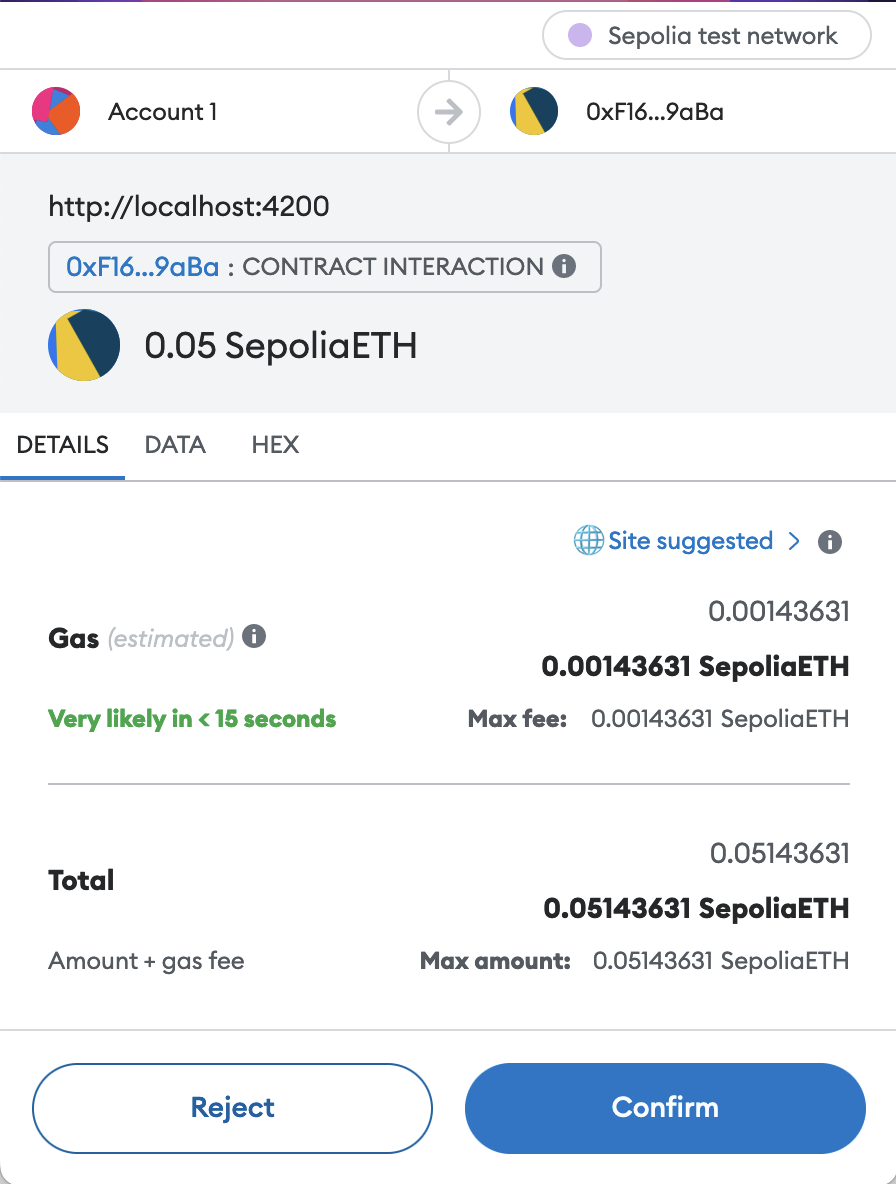
\includegraphics[width=0.9\linewidth]{src/img/checkout_metamask.png}
    \caption{Popup di pagamento su MetaMask}\label{fig:checkout_metamask}
    \end{subfigure}
    \begin{subfigure}{0.33\textwidth}
    \centering
    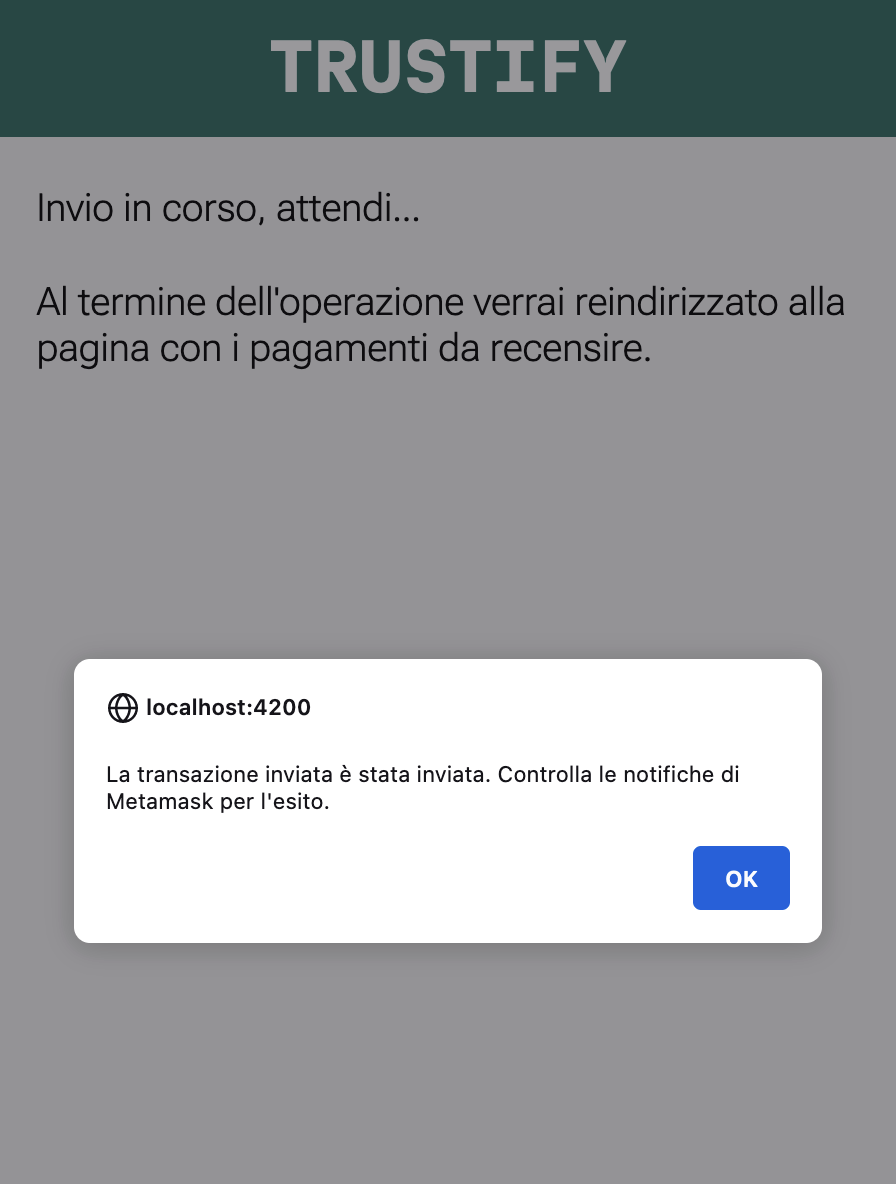
\includegraphics[width=0.9\linewidth]{src/img/checkout_conferma.png}
    \caption{Pagina di attesa e conferma pagamento}\label{fig:checkout_conferma}
    \end{subfigure}

    \caption{Checkout}\label{fig:checkout}
\end{figure}

\subsubsection{Login/Account}
Per effettuare il login, è necessario cliccare sul bottone "Login" e confermare l'accesso su MetaMask. Una volta effettuato il login, il bottone cambierà nome in "Account" e permetterà di visualizzare l'indirizzo del wallet utilizzato per l'accesso.

\begin{figure}[t]
    \begin{subfigure}{0.33\textwidth}
    \centering
    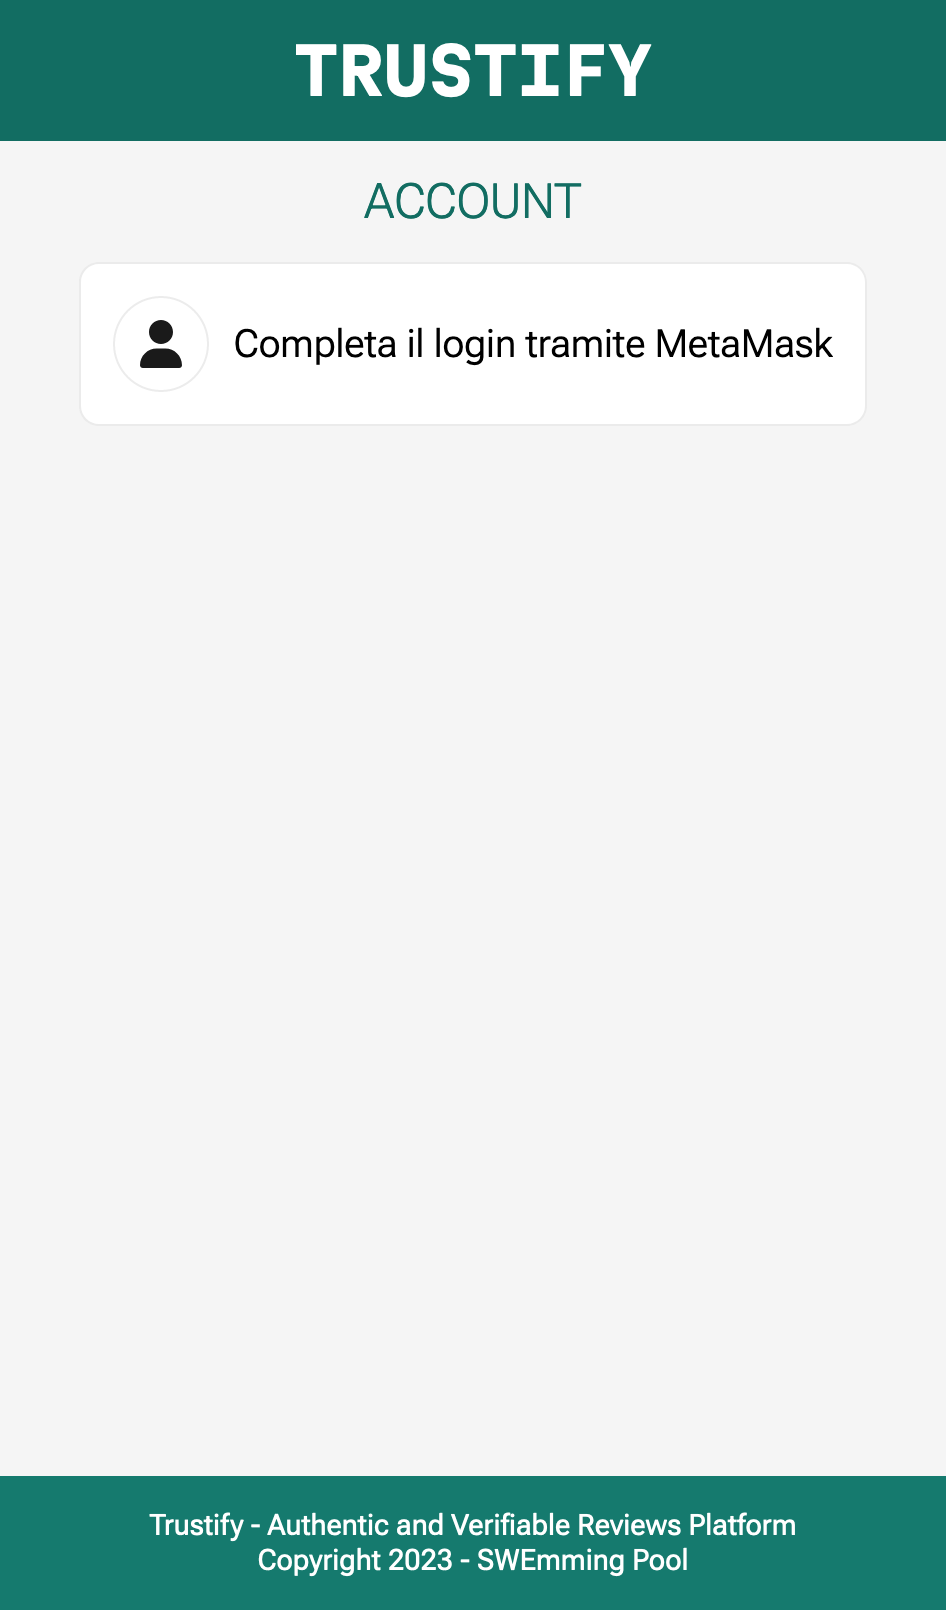
\includegraphics[width=0.9\linewidth]{src/img/login.png}
    \caption{Pagina di login}\label{fig:login_page}
    \end{subfigure}
    \begin{subfigure}{0.33\textwidth}
    \centering
    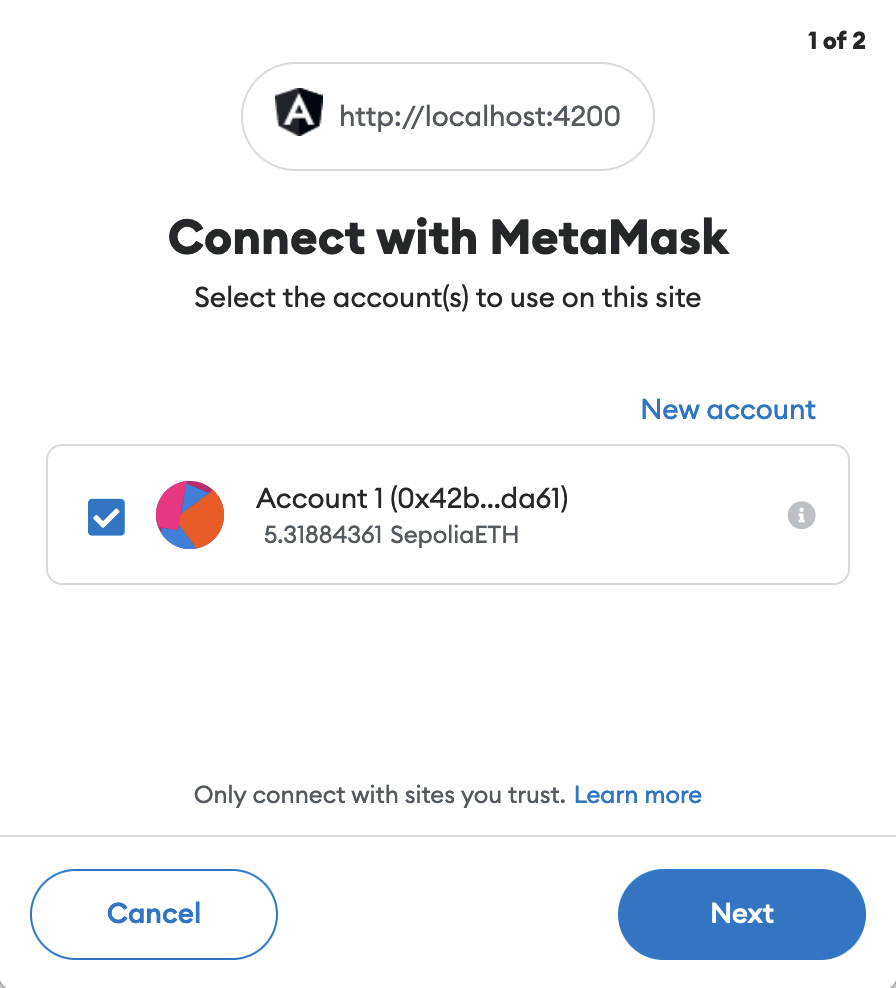
\includegraphics[width=\linewidth]{src/img/login_metamask.png}
    \caption{Popup di login su MetaMask}\label{fig:login_metamask}
    \end{subfigure}
    \begin{subfigure}{0.33\textwidth}
    \centering
    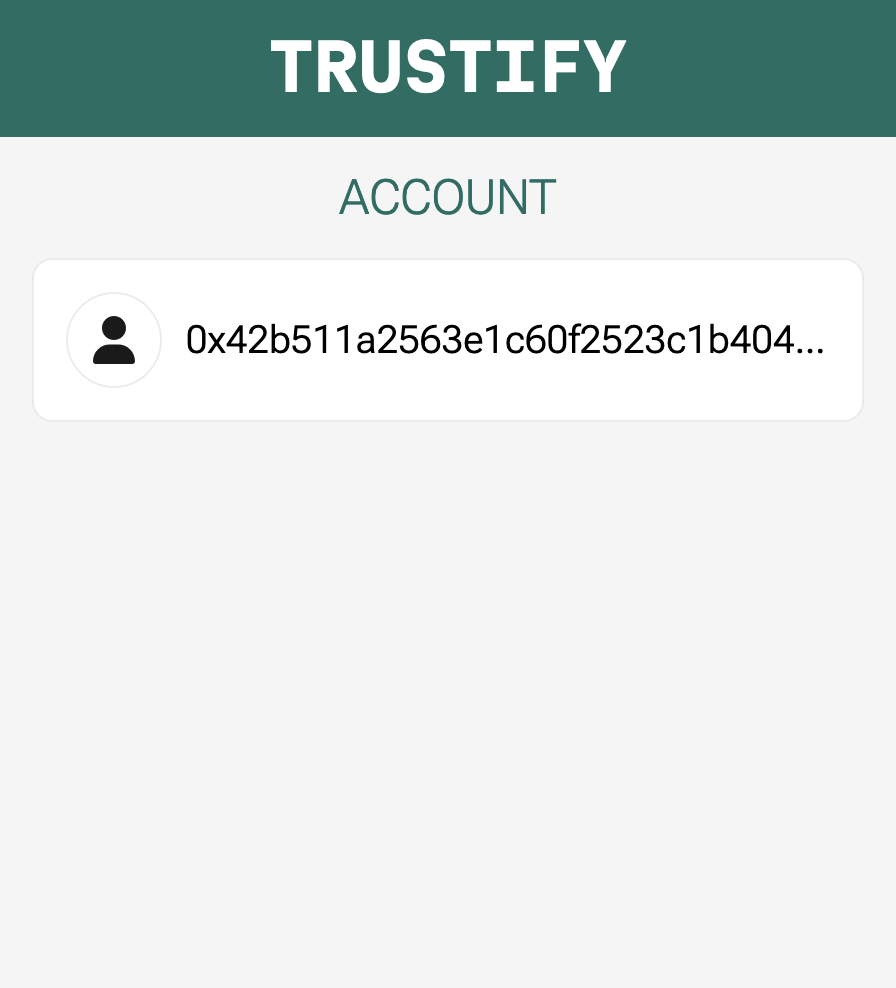
\includegraphics[width=\linewidth]{src/img/account.png}
      \caption{Pagina con l'indirizzo del proprio wallet}\label{fig:account}
    \end{subfigure}

    \caption{Login}\label{fig:login}
\end{figure}


\subsubsection{Pagamenti da recensire}
In questa sezione verranno visualizzati i pagamenti effettuati dall'utente che non sono ancora stati recensiti. Per ogni transazione, sarà possibile visualizzarne ID, indirizzo del destinatario, data e quantità di ether inviata, oltre ad un bottone per rilasciare una recensione. La seguente figura fa uso dei colori per evidenziare i differenti campi riportati per ogni transazione.
\begin{figure}
    \centering
    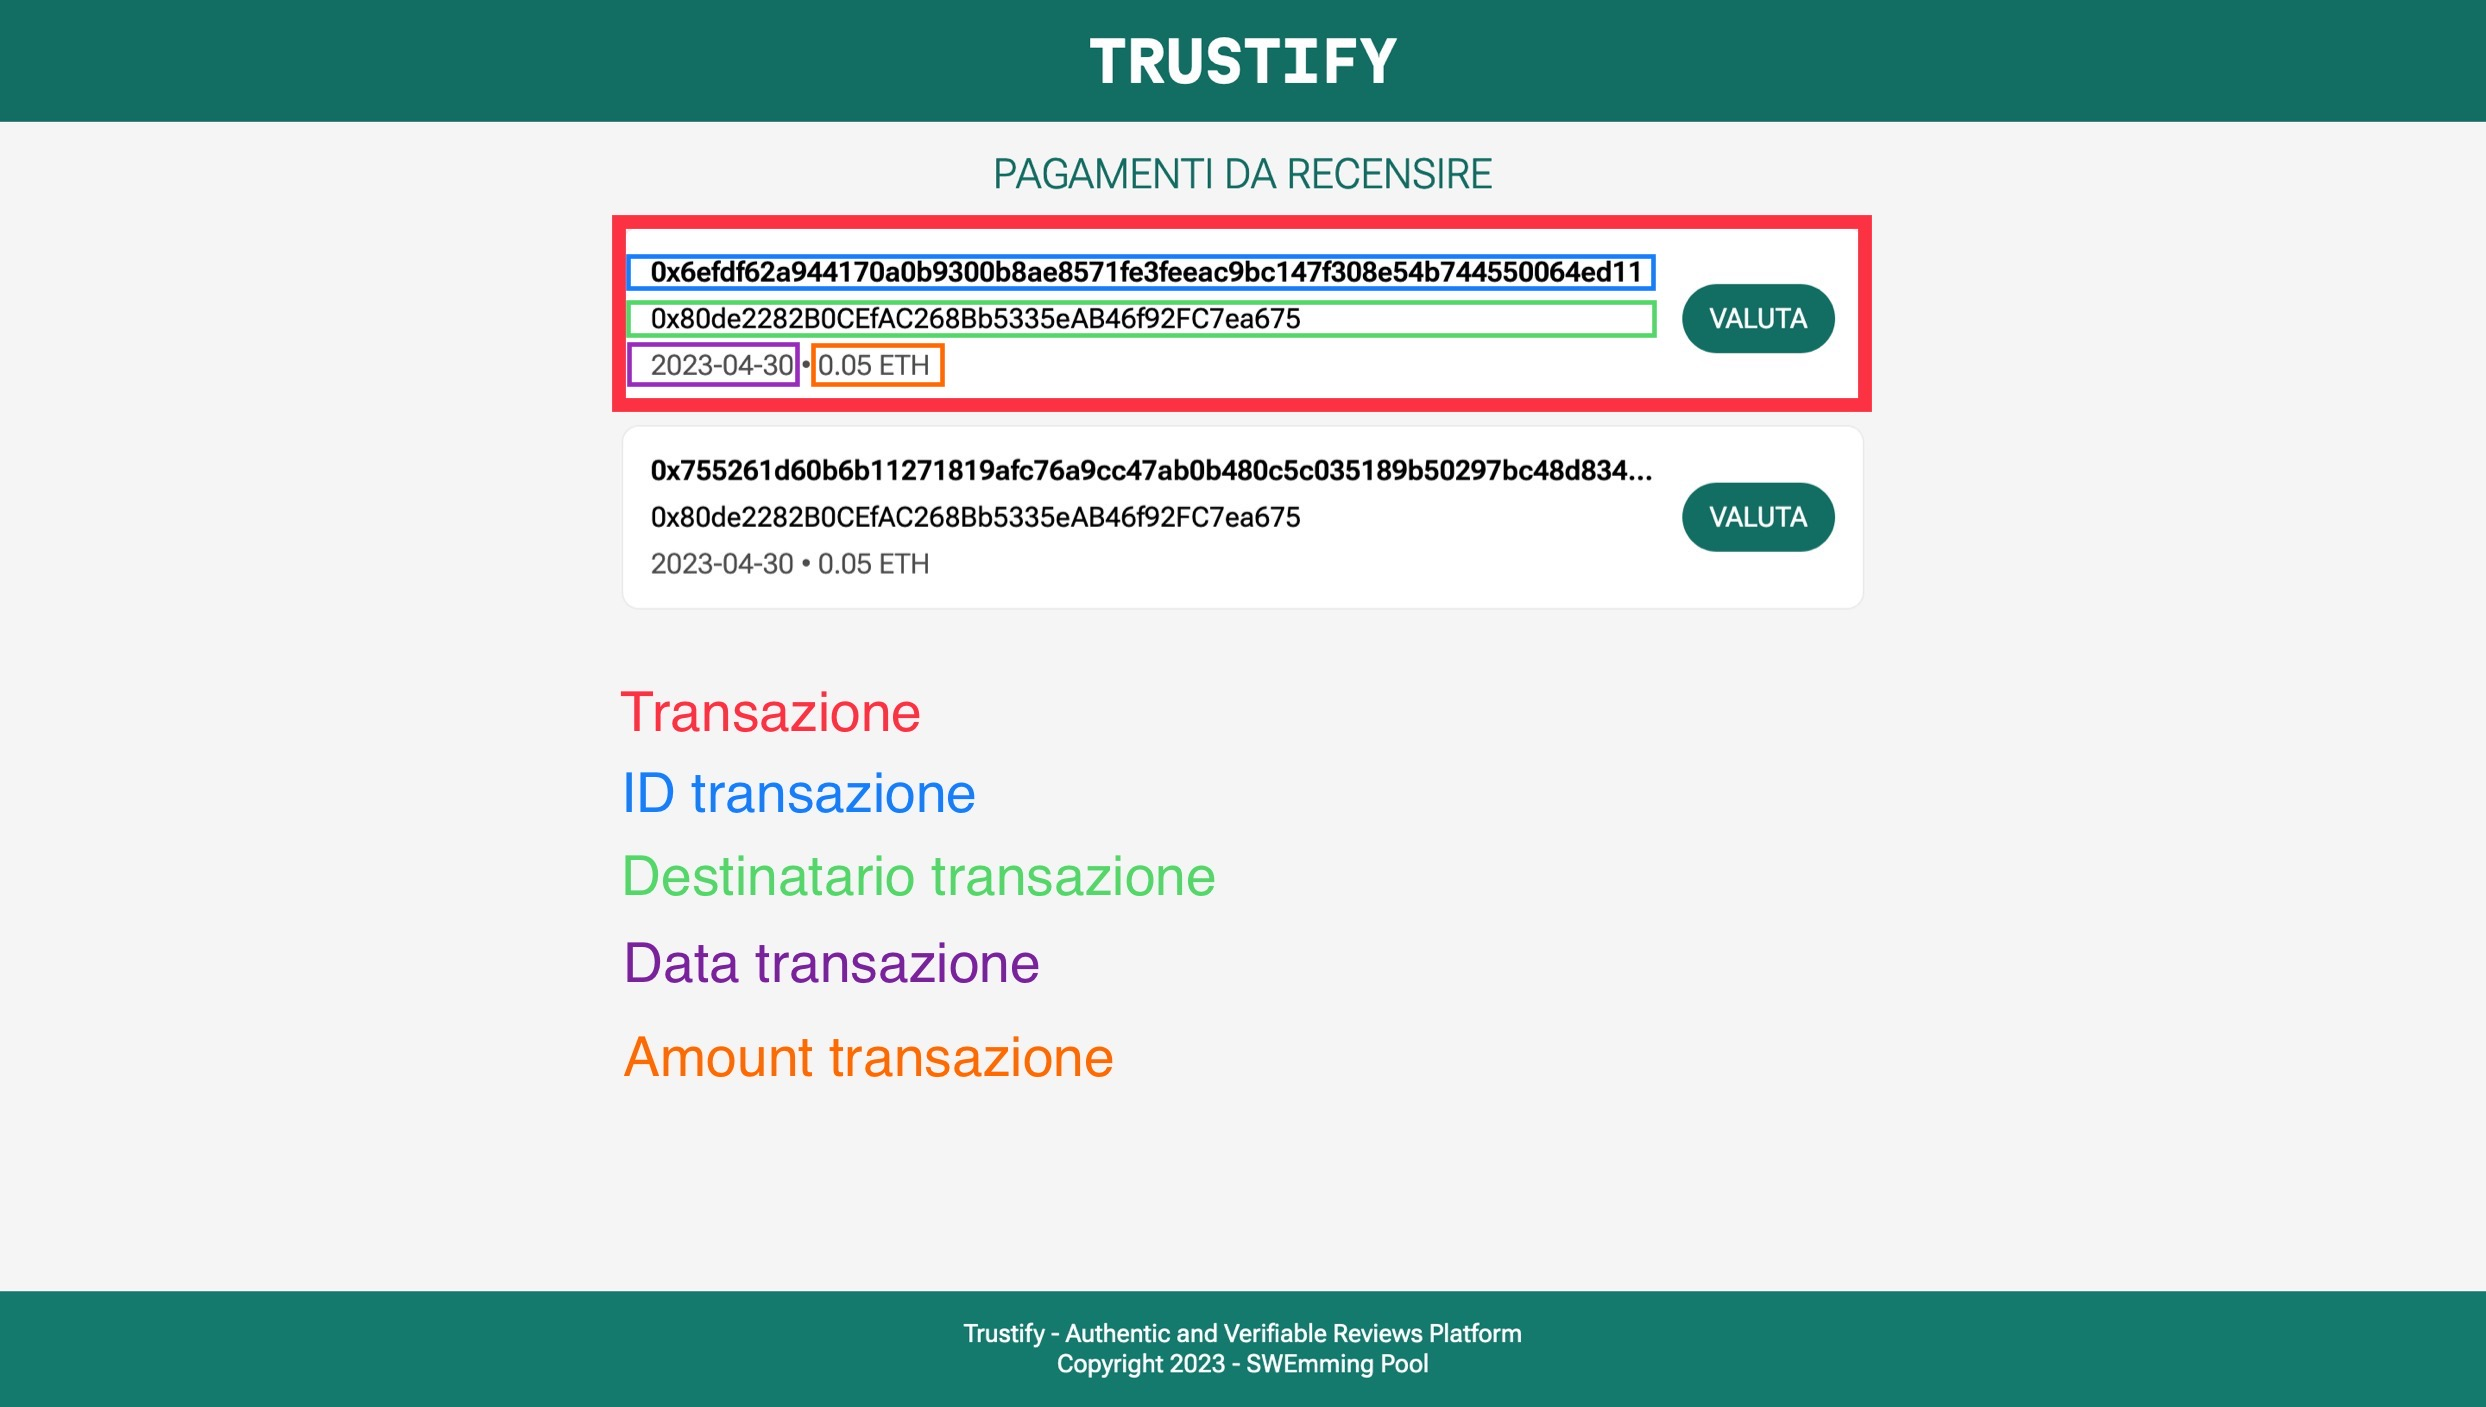
\includegraphics[scale=0.18]{src/img/pagamenti.jpg}
    \caption[Pagamenti da recensire]{Pagamenti da recensire\protect\footnotemark}\label{fig:pagamenti}
\end{figure}

\footnotetext{Per questioni di spazio, soprattutto nel layout mobile, non si sono inserite delle etichette per i campi, che potrebbero perciò risultare di difficile lettura; ipotizziamo però che, nella versione finale della web app, i vari indirizzi non saranno visualizzati in questo modo, ma saranno disponibili altre informazioni per identificare transazioni ed e-commerce.}

\subsubsection{Rilascio recensione}
In questa sezione sarà possibile rilasciare una recensione per un pagamento effettuato. In cima alla pagina sono visibili i dettagli della transazione, esattamente come avviene in \hyperref[fig:pagamenti]{Figura 9}; successivamente, bisognerà inserire un titolo, un punteggio da 1 a 5 e un commento. Una volta inseriti i dati, sarà possibile cliccare sul bottone "Invia" per confermare l'operazione.

Successivamente all'invio, sarà visualizzato un popup di MetaMask simile a quello in \hyperref[fig:checkout_metamask]{Figura 4} e una pagina di attesa e conferma simile a quella in \hyperref[fig:checkout_conferma]{Figura 5}.

\begin{figure}
    \minipage{0.45\textwidth}
      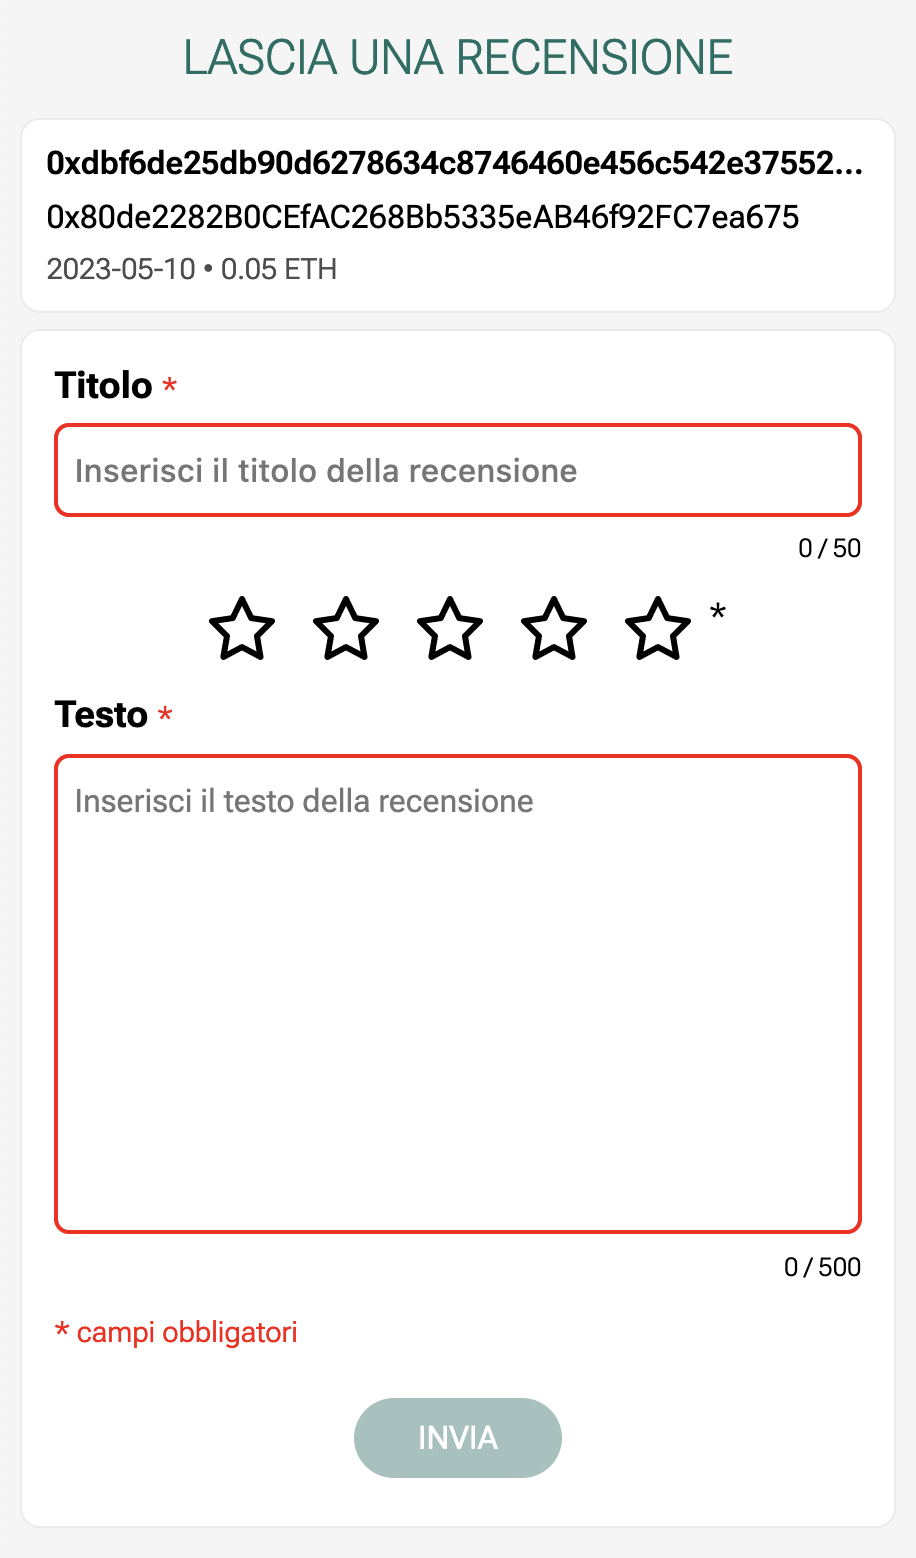
\includegraphics[width=\linewidth]{src/img/rilascio_recensione.png}
      \caption{Pagina rilascio recensione con campi vuoti}\label{fig:rilascio_recensione}
    \endminipage\hfill
    \minipage{0.45\textwidth}
      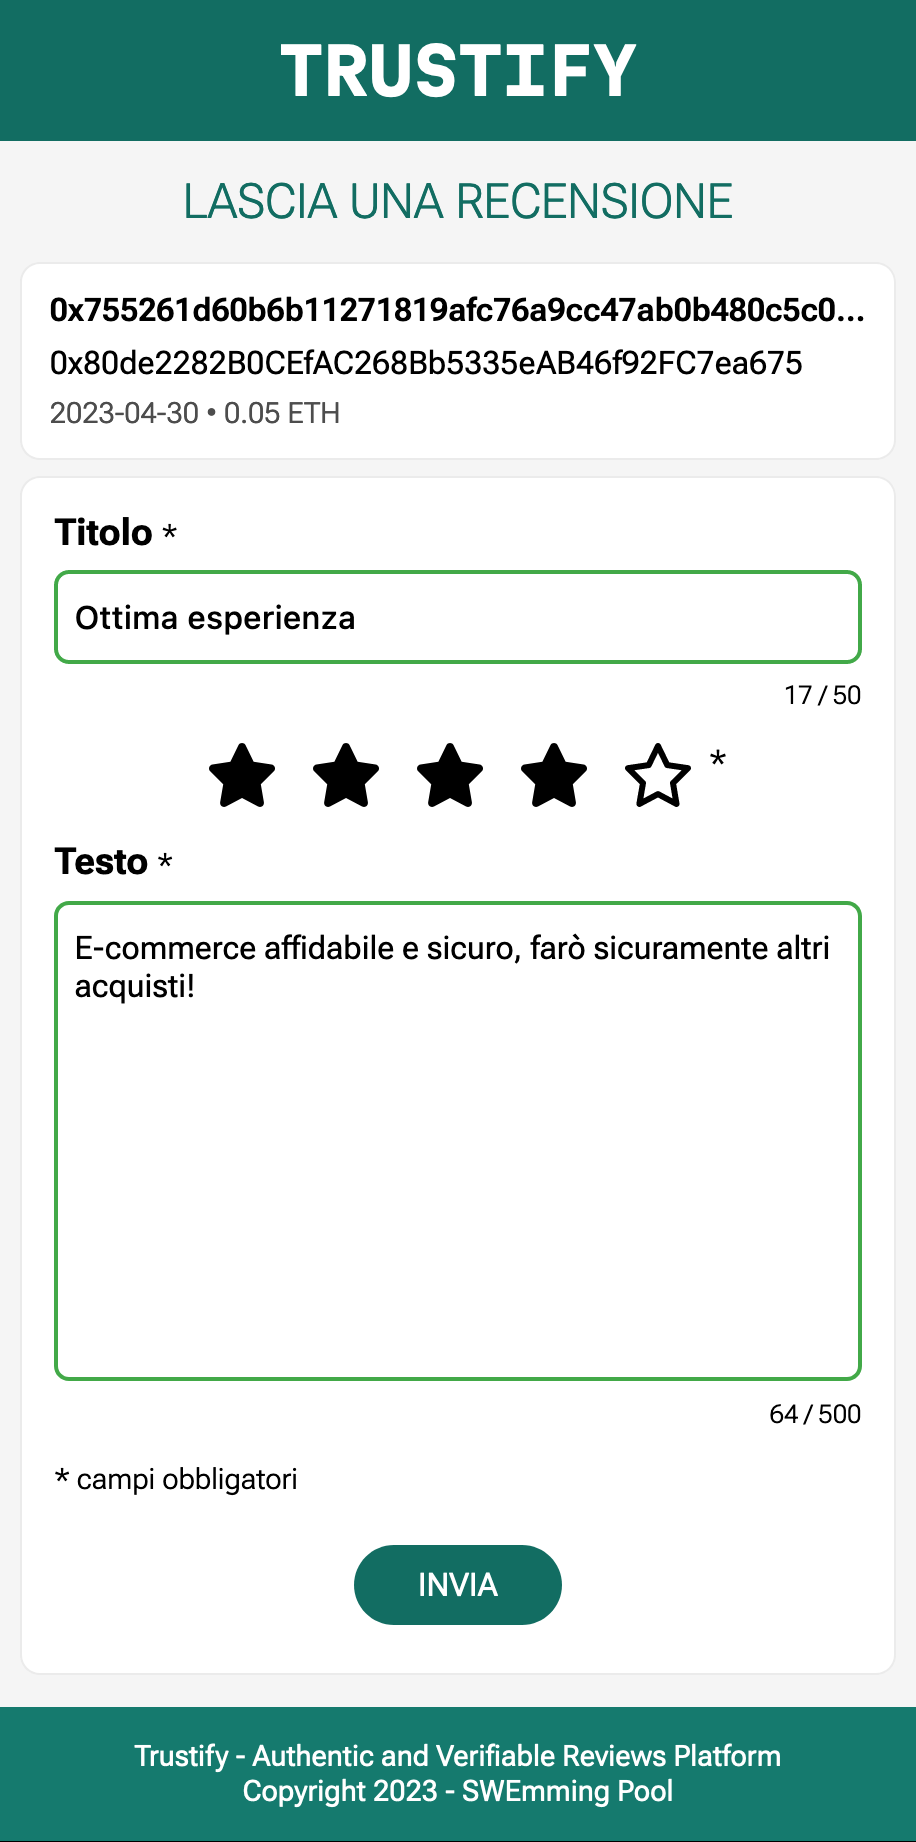
\includegraphics[width=\linewidth]{src/img/rilascio_recensione_valid.png}
      \caption{Pagina rilascio recensione con campi validi}\label{fig:rilascio_recensione_valid}
    \endminipage\hfill
\end{figure}


\subsubsection{Recensioni rilasciate e ricevute}
In queste sezioni è possibile visualizzare le recensioni rilasciate e ricevute dall'utente. Per ogni recensione, sarà possibile visualizzare il titolo, il voto e il commento, oltre ad alcuni dettagli della transazione. La seguente figura fa uso dei colori per evidenziare i differenti campi riportati per ogni recensione.

\begin{figure}
    \centering
    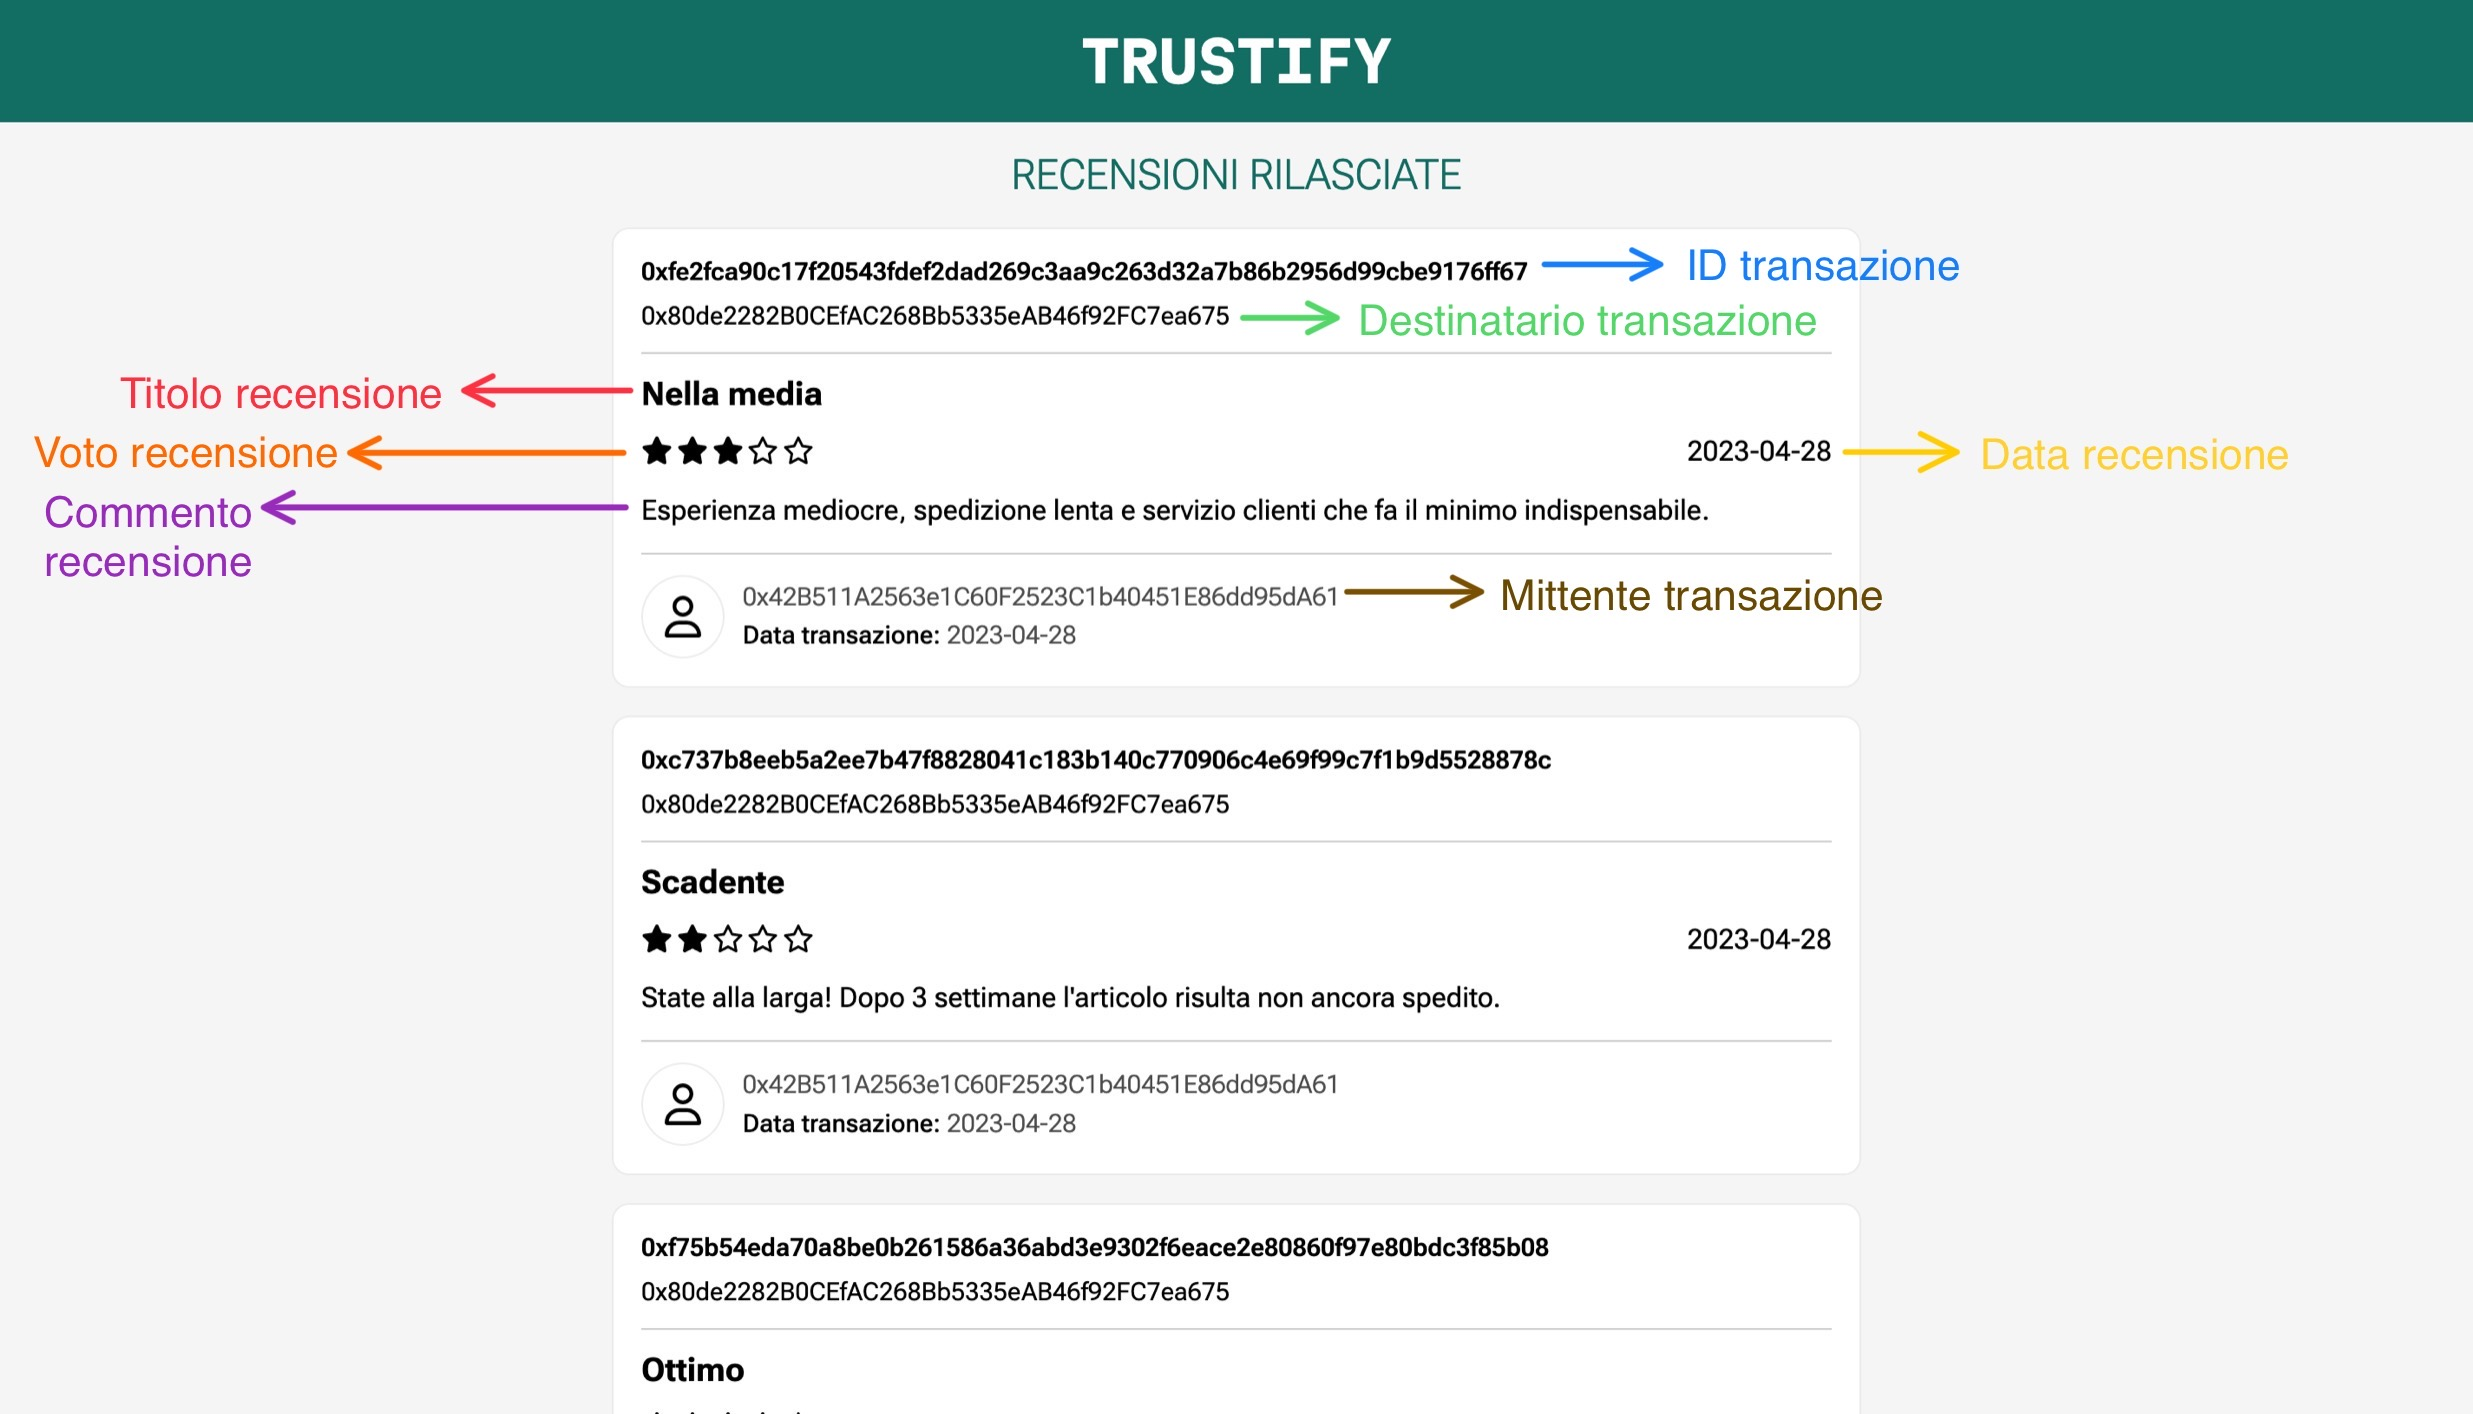
\includegraphics[scale=0.18]{src/img/recensioni_rilasciate.jpg}
    \caption{Recensioni rilasciate; la visualizzazione è la medesima per quelle ricevute}\label{fig:recensioni_rilasciate}
\end{figure}

\subsubsection{Ricerca recensioni}
Questa pagina, l'unica accessibile senza aver effettuato il login, permette di ricercare recensioni in base all'indirizzo del destinatario o dell'autore. La visualizzazione di ogni recensione è la stessa già mostrata in \hyperref[fig:recensioni_rilasciate]{Figura 12}.

\begin{figure}
    \minipage{0.45\textwidth}
      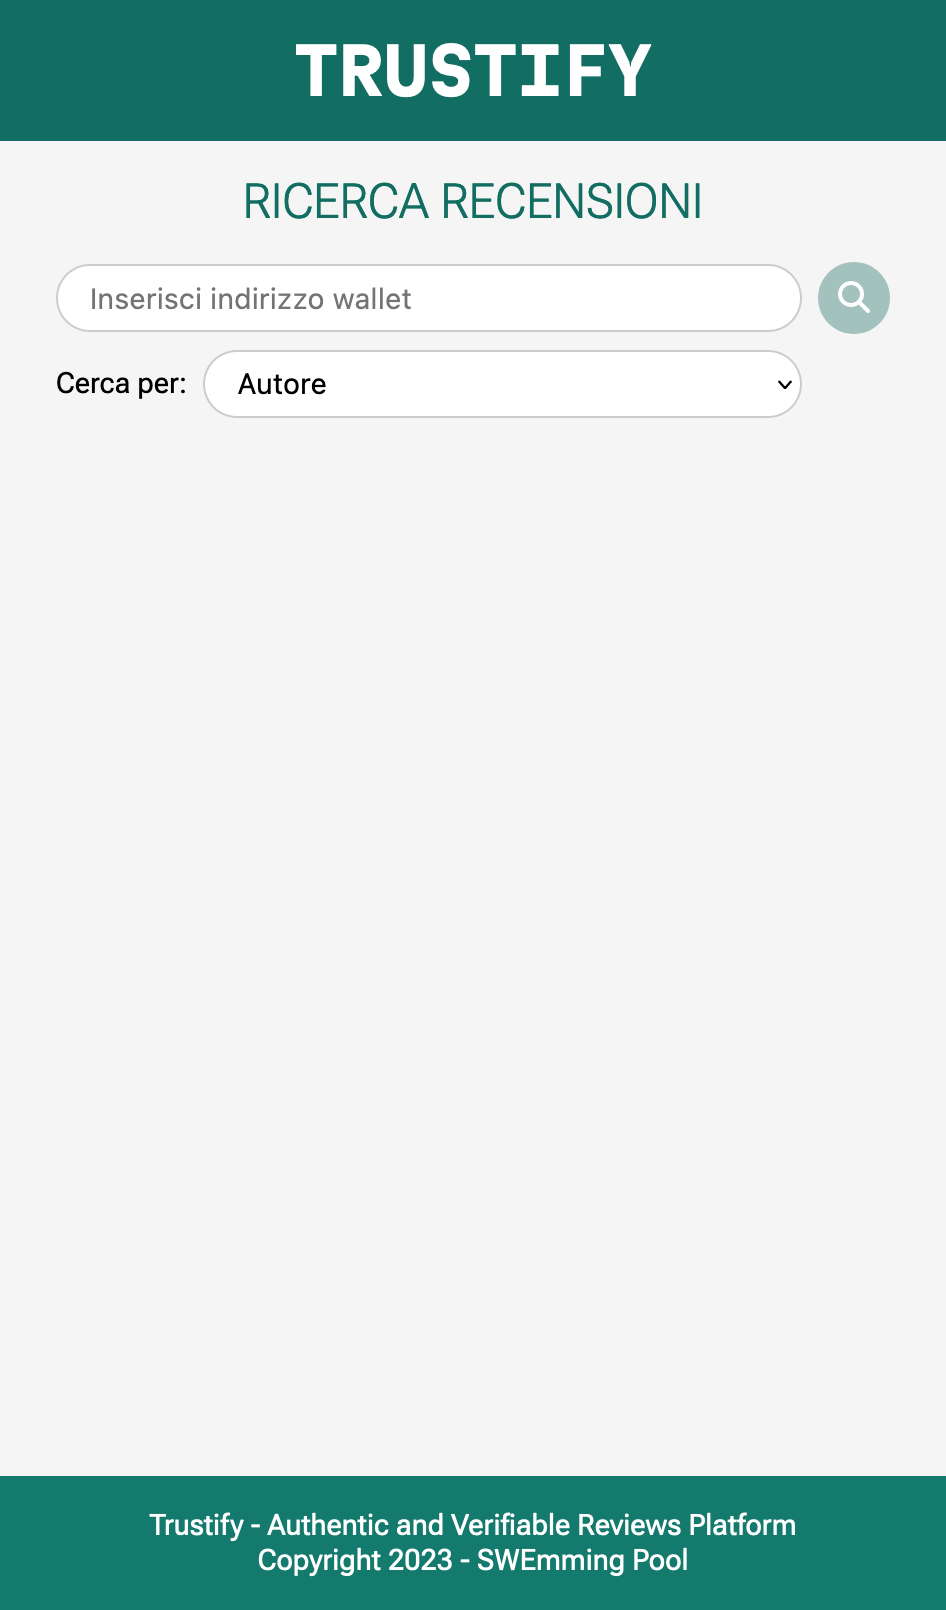
\includegraphics[scale=0.15]{src/img/ricerca_recensioni.png}
      \caption{Pagina ricerca recensioni con campo vuoto}\label{fig:ricerca_recensioni}
    \endminipage\hfill
    \minipage{0.45\textwidth}
      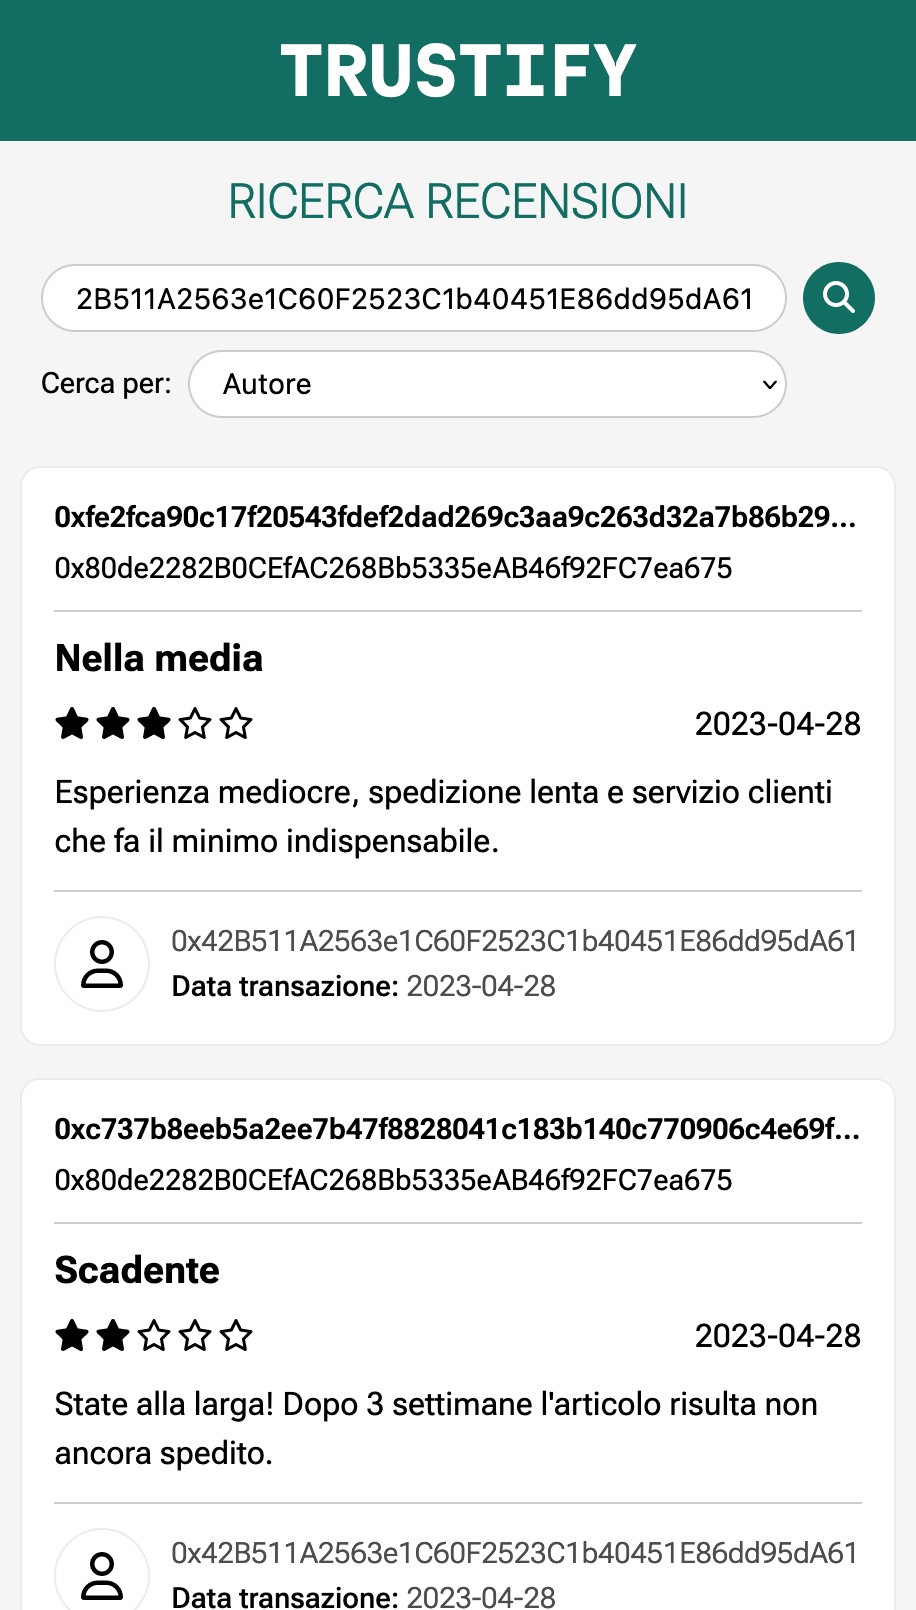
\includegraphics[scale=0.15]{src/img/ricerca_recensioni_valid.png}
      \caption{Pagina ricerca recensioni}\label{fig:ricerca_recensioni_valid}
    \endminipage\hfill
\end{figure}